\chapter{بررسی نحوهٔ فشرده‌سازی در فرمت JPEG}
\noindent
\textbf{
	\textit{
        توضیح نحوهٔ کار فشرده‌سازی در فرمت JPEG، 
        مقدمه‌ای بر DCT و 
        توضیح کلی 
        \lr{Huffman encoding}
	}
}
\pagebreak

\section{DCT}

\subsection{
تعریف 
}

تبدیل کسینوسی گسسته (به انگلیسی:
 \lr{Discrete cosine transform})
 ، دنباله‌ای محدود از اعداد (داده ها) را به‌ صورت مجموع توابع کسینوسی با فرکانس های متفاوت نمایش می‌دهد.
 تبدیل کسینوسی گسسته، شباهت بسیاری به تبدیل فوریه گسسته (DFT) دارد، با این تفاوت که حاصل تبدیل فقط مقادیر حقیقی دارد (بر خلاف تبدیل فوریه که منجر به مقادیر مختلط می شود).

 به صورت علمی‌تر می‌توان نوشت که 
 DCT 
 تابعی معکوس‌پذیر و خطی از 
 $R^N$ 
 به 
 $R^N$
 است.

 فرمول کلی DCT 
 برای فضای یک‌بعدی به شکل زیر است.

 \begin{equation}
 X_k = \sum_{n = 0}^{N - 1} x_n \cos [\pi / n  (n + 1/2)k]
 , k = 0, ..., N - 1
 \end{equation}

 \section{تبدیل دنباله‌ای از پیکسل‌ها به تابع}
هر تصویر در حقیقت به صورت چهار ماتریس دوبعدی ذخیره می‌شود که هر ماتریس مقدار رنگی پیکسل را برای آن کانال رنگی
(RBG و $\alpha$)
نشان می‌دهد، برای کمپرس کردن یک عکس ماتریس‌های کانال‌های رنگی مختلف را جداگانه فشرده می‌کنیم، کانال رنگی R 
را در نظر بگیرید، در این حالت یک ماتریس 
$n * m$ 
داریم که هر خانهٔ آن عددی بین ۰ تا ۲۵۵ را نشان می‌دهد، برای سادگی یک سطر از این ماتریس را در نظر بگیرید، این سطر معادل با یک 
آرایه از اعداد می‌باشد، در صورتی که تمامی اعداد را از دامنه ۰ تا ۲۵۵ به دامنه ۱۲۸- تا ۱۲۷ ببریم می‌توانیم این دنباله را با مجموعه‌ای از 
توابع کسینوسی بازتولید کنیم، این ضرایب همان ضرایبی‌ست که با استفاده از DCT 
می‌خواهیم به دست بیاوریم.

شکل
\ref{freq_1}
نمونه‌ای از توصیف عکس با توابع کسینوسی را نشان می‌دهد.

حال اگر دو تابع نشان‌داده شده در 
شکل 
\ref{freq_1}
 
را با هم جمع کرده و میانگین بگیریم، به نمایش فرکانس دیگری می‌رسیم که در شکل 
\ref{freq_2}
نشان داده شده است.
در صورتی که به شکل‌های متفاوت و با ضرابت متفاوت توابع مختلف کسینوسی را با هم جمع کنیم می‌توانیم هر فرکانسی را بسازیم. این کاری‌ست که در 
عمل الگوریتم 
DCT برای ما انجام می‌دهد.
\begin{figure}[]
        \centering
        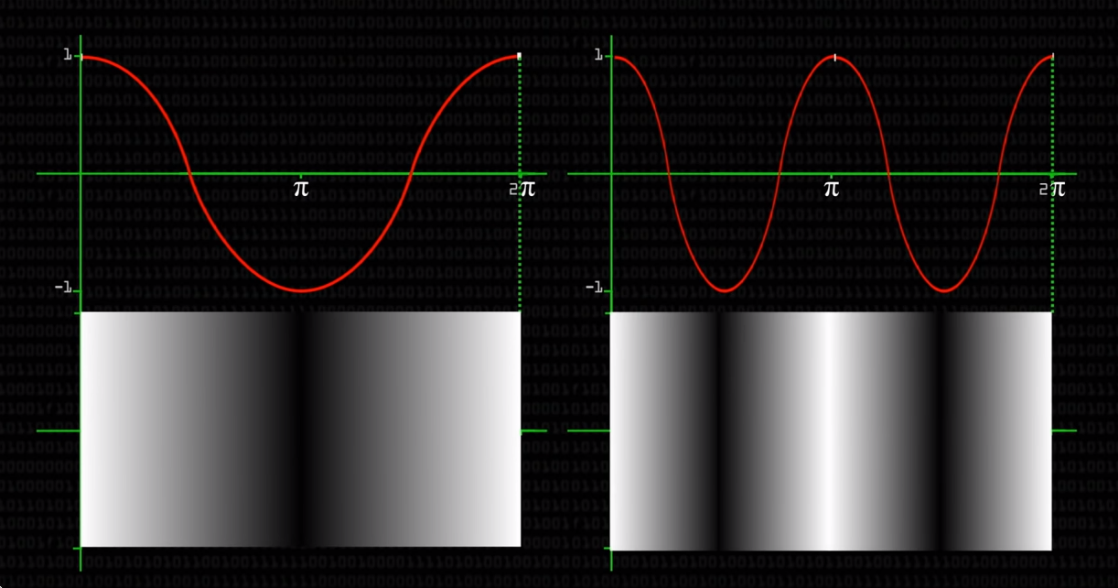
\includegraphics[width=\textwidth]{figs/freq_1.png}
        \caption{توصیف فرکانسی توابع 
        $\cos (x) , \cos (2x)$ }
        \label{freq_1}
\end{figure}

\begin{figure}[]
        \centering
        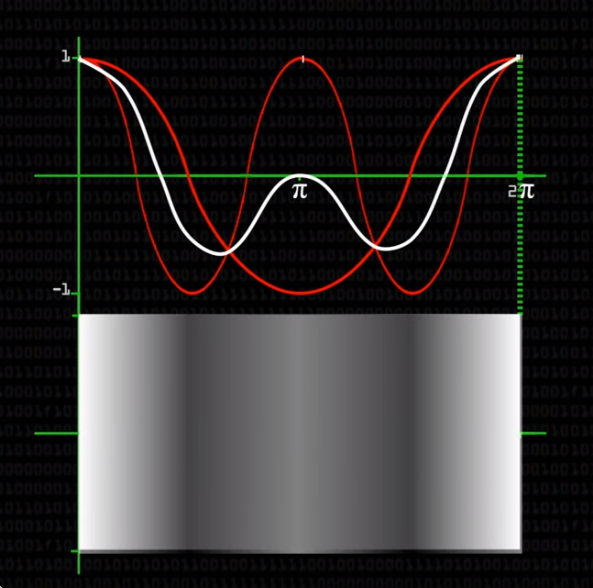
\includegraphics[width=0.5\textwidth]{figs/freq_2.png}
        \caption{توصیف فرکانسی تابع 
        $\cos (x) + \cos (2x)$}
        \label{freq_2}
\end{figure}

\section{نحوهٔ کار JPEG}
برای فشرده‌سازی یک تصویر در JPEG 
مراحل زیر انجام می‌شود. 

\begin{itemize}
        \item تبدیل تصویر به بلوک‌های کوچک 
        \item تبدیل هر بلوک به مجموعه‌ای از توابع کسینوسی استاندارد با DCT
        \item تنظیم ضرایب متناسب برای بلوک‌های DCT 
        \item کمپرس کردن ضرایب با استفاده از Huffman
\end{itemize}